\section*{Problem 2}
\addcontentsline{toc}{section}{Problem 2}

\textbf{Statement:}

The point is seleted in random at unit circle and then projected to the diameter.
Find the probability that the distance from the origin is more than $\frac{1}{2}.$

\noindent\textbf{Solution:}

We assume that the point is selected uniformly at the unit circle, and that the
diameter is the $x$ axis.

Note that to project a point to the diameter we can just take the $x$ coordinate
of the point.

So the points with $x$ coordinate less than $-\frac{1}{2}$ or greater than
$\frac{1}{2}$ are the points that are more than $\frac{1}{2}$ away from the origin.

Let's plot the unit circle with this two set of points:

\begin{figure}[H]
    \centering
    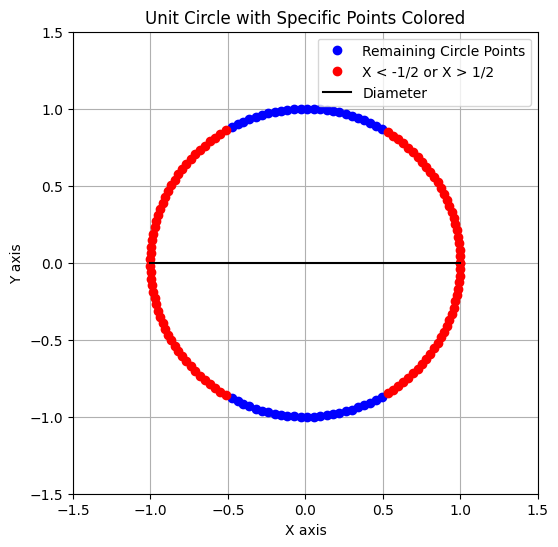
\includegraphics[width=0.5\textwidth]{images/unit-circle.png}
\end{figure}

So we can solve this problem by finding the perimeter of the unit circle made by
red points and divide it by the perimeter of the unit circle.

The perimeter of the unit circle is $2\pi$, so we need to find the perimeter of
the unit circle made by red points.

To find the perimeter of the unit circle made by red points we can find the following angle:


\begin{figure}[H]
    \centering
    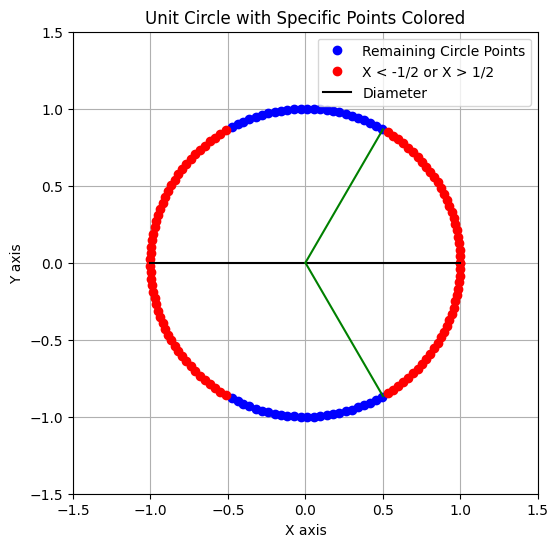
\includegraphics[width=0.5\textwidth]{images/unit-circle-angle.png}
\end{figure}

And then multiply by two to get the total sum of the angles that conform the
arc of the unit circle made by red points.

It can be notice that the angle is just $2 \cdot acos(\frac{1}{2})$ and then multiply
by two to get the total sum of the angles that conform the arc of the unit circle

But we can notice that the length of any angle is the same as the length of the arc define by the angle (because this is a
unit circle).

So the perimeter of the unit circle made by red points is $4 \cdot \text{acos}(\frac{1}{2})$.

So the probability is:

\begin{equation*}
    P( \text{distance from origin} > \frac{1}{2} ) = \frac{4 \cdot \text{acos}(\frac{1}{2})}{2\pi} = \frac{2 \cdot \text{acos}(\frac{1}{2})}{\pi} = \frac{2 \cdot \frac{\pi}{3}}{\pi} = \frac{2}{3}
\end{equation*}